 \mysection{The Night Child}{species-night-child}


  \flavor{\myital{
    "Lie close," Laura said, \\
    Pricking up her golden head:\\
    "We must not look at goblin men,\\
    We must not buy their fruits:\\
    Who knows upon what soil they fed\\
    Their hungry thirsty roots?"\\
    "Goblin Market", Christina Rossetti
    }
  }


  \mysubsection{Me Handsome!}{night-child-appearance}

  Other folk? Not smart like we are (maybe Pooka, not sure).  They dumb, just pretend they know.  Only we know truth - Life and Chaos are same-same.  And no one talk to Chaos the way \myital{we} do. Humans say that make us bad. "One hole owed" they say.  But we owe nothing! Plus you can't owe a hole. Hole not there! See how dumb they are? Only real way talk to Chaos is be Chaos.  Chaos all around, like ocean. Folks build boats.  We swim.  That make us strong. That make us wise.


  \mysubsection{Basics}{night-child-basics}

  \myhighlight{Me Strong!}{night-child-flesh}

  Night Children have a d10 \FLESH
  
  
  \myhighlight{Me Clever!}{night-child-clever}

  You add your \LVL to any \RO or \RB attempt that includes your Talent.  The \UD still moves \DCDOWN on a natural 1 or 2.


  \mysubsection{Bad Stuff}{night-child-complications}

    Get bad news out of the way!

  \myhighlight{Me Tiny!}{night-child-complication-tiny}
  
  You stand only 1m tall to start.  You can only carry a number of Significant Items equal to your \MAX \VIG (you don't get the +2 bonus). If you wear armor, you can only wear armor for "little people" (child-sized).  You cannot wield 2-handed weapons.

  \cbreak

  \myhighlight{No Talk Good!}{night-child-complication-no-talk-good}

  Speak in words of 2 syllables or fewer.

  \myhighlight{One Hole Owed!}{night-child-complication-unhallowed}

  You have no "soul" and are Unhallowed. You can't enter consecrated ground and are affected by the Mystic ability "Curse the Unhallowed"


  

  \mysubsection{Make Me!}{night-child-creation}


  \callout{
    \mynumlist {
      \item One core Skill is \DCUP!
      \item One Save is \DCUP!
      \item Talent is \DCUP! (now a d8)
      \item Grab 3 d6 - time to see what we do!
    }
  }


  \mysubsection{Virtues}{night-child-virtues}

  Night Children have 3 core Virtues:  Weird, Looks, and Gear.  Each Virtue starts at a single d6; roll these d6 at character creation to determine your starting Weird, Looks, and Gear. Add the 3 d6 up to determine your Snag

  As you go up in level, you have the opportunity to move your Looks, Gear, and/or Weird \DCUP - and to roll additional Virtues. See the section on \mylink{Advancement}{advancement}. 

  \mybold{Starting Gear}: In addition to your Gear roll below, you start with:

  \mybullet {
    \item half a pair of scissors (dagger) and a big stick (club);
    \item 5 useless items (wad of used tissues, taxidermied toad, etc)
  }


  \newpage


  \end{multicols}




  \mytable{l X X X}{
    \thead{Roll} & \thead{Weird} & \thead{Looks} & \thead{Gear} \\
  }{
        1 & Bug Barf & Fishy & Bedlam Bag \\
        2 & Crafty & Glass Teeth & Big Helm \\
        3 & Gassy & Owl Eyes & Big Shield \\
        4 & Run Away & Rat Tail & Bug Pal \\
        5 & Shocky & Spider Eyes & Devil Pen \\
        6 & Spin Silk & Sticky & Gobbomb \\
        7 & Anklebiter  & Bat Ears & Gobsword \\
        8 & Twitchy & Tusky & Trunk Pal \\
        9 & Bad Blood & Frog Mouth & Little Buddy \\
        10 & Shedding & Pig Snout & Skelly Key \\
        11 & Bad Spit & Harpy Claws & Big Pal \\
        12 & Rando & Rooty & Gremlin Tools \\
        13 & Bloodthirst & Bigg'un & Bogeylatch \\
        14 & Bouncy & Camo & Kazoo \\
        15 & Crazy & Skin Bag & Magic Beans \\
        16 & Meat on Menu & Tough'un & Mirror Mirror \\
        17 & Big Boom & Fly Wings & Hole \\
        18 & Eat Brains & Goo & Kissy Lips \\
        19 & Nose Hairs & 'nother Arm & Red Shoes \\
        20 & Wut? & Shell & Spinny Wheel \\
        21 & Bad Breath & Babies! & Fly Rug \\
        22 & Sleepy & Beardy & Packpack \\
        23 & Troll Blood &  Smoky & The Crew \\
        24 & Me Human! & Lie Can & Vorpal Sword \\ 
  }

  \mybold{Snags} (total of Weird, Looks, and Gear)

  \mytable{l X l X l X}{
    \thead{Roll} & \thead{} & \thead{Roll} & \thead{} & \thead{Roll} & \thead{} \\
      3 & Angry & 9 & Glowy & 15 & Smell Yummy \\
      4 & Backwards & 10 & Me Cold! & 16 & Stealy \\
      5 & Bad Mouth & 11 & Me Hot! & 17 & Weird Voice \\
      6 & Bumpback & 12 & Me Hungry! & 18 & Who That? \\
      7 & Dirty & 13 & Me Tired ... & - & - \\
      8 & Fat & 14 & Pinhead & - & - \\
  }
      

  \callout {
    Weird and Looks get more powerful the more times you roll the result. See the description for details.
    ~\\
    ~\\
    Gear is unique.  If you roll a result you've rolled before, roll again.
  }


  \newpage


  \begin{multicols}{2}
  \raggedcolumns


  \mysubsection{Weird}{night-children-virtues-weird}

  \mybold{Anklebiter}
  \mylist {
    \item 1st time: You deal +1 damage
    \item 2nd time: You deal +4 damage
    \item 3rd time: You deal +\LVL damage
    \item 4th or more: Roll again
  }

  \mybold{Bad Blood}
  \mylist {
    \item 1st time: Your blood is acidic. When enough of your blood mixes with air (that is, outside your body), it becomes an Iron acid.  You need to bleed about a pint of blood for it to work.  Bleeding more doesn't increase the effectiveness.
    \item 2nd time: As above, but it's a Silver acid
    \item 3rd time: As above, but it's a Gold acid
    \item 4th or more: Roll again
  }

  \mybold{Bad Breath}
  \mylist {
    \item 1st time: Once per Session, you can breathe out a cone of fire, acid, frost, etc (your choice).  The breath does 3d6 damage, Save vs. Doom for half damage.
    \item 2nd time: As above, but you deal 5d6 damage
    \item 3rd time: As above, but you deal \LVL d6 damage
    \item 4th or more: Roll again
  }

  \mybold{Bad Spit}
  \mylist {
    \item 1st time: Your saliva is toxic in high enough quantities.  Once per Session, you can spit out a dram or so of liquid that acts as an Iron toxin.  Treat this toxin as an Unguent.
    \item 2nd time: As above, but it's a Silver toxin
    \item 3rd time: As above, but it's a Gold toxin
    \item 4th or more: Roll again
  }

  \mybold{Bloodthirst}
  \mylist {
    \item 1st time: If a Monster is already injured (has taken damage to Flesh), deal +1 damage.  Stacks with Anklebiter.
    \item 2nd time: As above, but +3 damage
    \item 3rd time: As above, but +5 damage
    \item 4th or more: Roll again
  }


  \mybold{Big Boom}
  \mylist {
    \item 1st time: You can explode.  This will absolutely kill you.  Everyone Close to you must Save vs Doom or immediately perish; everyone Nearby to you must Save vs Doom or fall to 0 Flesh.
    \item 2nd time: Roll again
  }

  \mybold{Bouncy}
  \mylist {
    \item 1st time: You can fall up to 10m without any negative effect (unless you fall into lava or something)
    \item 2nd time: You can fall any distance without negative effect (unless you fall into lava or something)
    \item 3rd time: You can "bounce" up to half the distance you've fallen.  For example, if you fall 10m, you can then "bounce" 5m up.  If you're trying to bounce up to something else, common sense prevails about the angle and the material of the thing you're bouncing off of.
    \item 4th time: Roll again
  }



  \mybold{Bug Barf}
  \mylist {
    \item 1st time: One per Session, barf up big sack of spiders, worms. Feed up to 6 friends
    \item 2nd time: As above, but you can barf the spiders and bugs into a wound to cauterize it.  Immediately remove any Bleeding effects or infections.
    \item 3rd time: As above, but the spiders and bugs also have healing properties when you eat them.  Everyone who partakes heals your \LVL Flesh
    \item 4th time: Roll again
  }


  \begin{center}
  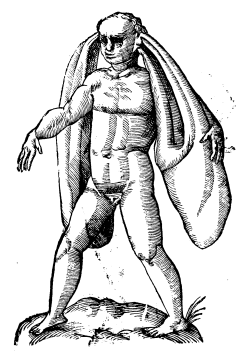
\includegraphics[scale=.5]{Goblin_1}
  \end{center}

 


  \mybold{Crafty}
  \mylist {
    \item 1st time: You gain the Skill: Tinker at \mybold{Trained (d8+1)}
    \item 2nd time: You gain the Skill: Tinker at \mybold{Skilled (d12+2)}.  If you're already Skilled, roll again.
    \item 3rd time: You gain the Skill: Tinker at \mybold{Master (d20+3)}.  If you're already a Master, roll again
    \item 4th time: Roll again
  }


  \mybold{Crazy}
  \mylist {
    \item 1st time:  If you fail a Sanity roll, roll a Save vs. Doom.  If you succeed, you don't need to roll on the \mylink{Terrifying Tables}{misc-terrifying-tables}
    \item 2nd time:  You are immune to Madness of all sorts
    \item 3rd time:  Roll again

  }


  \mybold{Eat Brains}
  \mylist {
    \item 1st time:  If you eat a sorcerer's brain, you learn all of the spells that they have written in their skulls.  These spells become a part of you; you can cast them at will using your Talent \UD
    \item 2nd time:  Roll again
  }

  \mybold{Gassy}
  \mylist {
    \item 1st time: You can emit a foul smelling gas that causes Disgust to everyone Close except you (no Save). This affects friends and foes alike. The smell lasts for Minutes.
    \item 2nd time: As above, but the smell also prompts a Sanity check
    \item 3rd time: As above, but the gas also ignites in open flame, dealing 4d6 damage to everyone Close (Save vs Doom for half damage)
    \item 4th time: Roll again
  }

  \mybold{Meat on Menu}
  \mylist {
    \item 1st time: You can pretty much eat anything without getting sick.  If you eat something with flesh (dead or otherwise) during a Breather, you regain an additional d6 Grit; if you eat something with flesh (dead or otherwise) when taking a \mylink{Bivouac}{combat-resting-bivouac}, you don't need to roll your \UD for Provisions.  
    \item 2nd time:  [Breather]: As above, but heal your Grit to \MAX; [Bivouac] Restore an extra \UD of any \myital{one} \mylink{Intangible Stat}{intangible-stats}
    \item 3rd time:  Roll again
  }

  \mybold{Nose Hairs}
  \mylist {
    \item 1st time:  Your nose hairs filter out any airborne toxins, rendering you immune
    \item 2nd time:  As above, but you can form toxic boogers out of the toxin.  By picking these out of your nose, you can get 1 d4 \UD of the toxin that was used on you
    \item 3rd time:  As above, but you can now flick these boogers.  Treat as if they were Thrown weapons that deal 1 point of damage, plus the effect of the Toxin if they strike flesh
    \item 4th time:  Roll again
  }


 \mybold{Go Night Night}
  \mylist {
    \item 1st time: Once per Session, when taking a \mylink{Bivouac}{combat-resting-bivouac}, you wrap yourself in a cocoon.  You are completely helpless in this state.  When you emerge (a) your Grit and Flesh are completely restored; (b) your \UD for all Intangible Stats are set to their \MAX; and (c) all Physical Wounds are removed
    \item 2nd time: Roll again
  }


  \mybold{Spin Silk}
  \mylist {
    \item 1st time: Once per Session, you can spin up to 25m of silk rope out of ... a place.
    \item 2nd time: As above, plus: once per Session, you can "shoot" webs out of your ... out of the place.  Creatures struck by the webs are stuck (treat as Paralyzed) unless they Save vs Doom.  The effect lasts for d4 Markovian.  The webs are extremely flammable.
    \item 3rd time: As above, except the webs last for d12 Markovian
    \item 4th time: Roll again
  }

  \mybold{Troll Blood}
  \mylist {
    \item 1st time: You can regenerate 1 Flesh over Hours (preventing you from Dying), unless the damage is from fire, acid, or magic (including magic weapons).
    \item 2nd time: As above, plus:  at the end of Combat, when you take a Breather, you heal \LVL Flesh
    \item 3rd time: As above, except: you regenerate 1 Flesh at the top of every Moment.
    \item 4th time: Roll again
  }


 \mybold{Twitchy}
  \mylist {
    \item 1st time: Add +4 to your Init rolls
    \item 2nd time: You always win Init (like a Pooka)
    \item 3rd time: Roll again
  }

  \begin{center}
  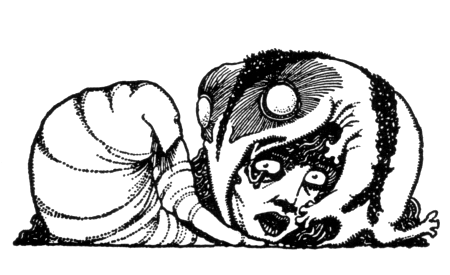
\includegraphics[scale=.5]{Goblin_2}
  \end{center}



  \mybold{Me Human!}
  \mylist {
    \item Every time: You can take a Virtue from any Mortal Trope
  }

  \mybold{Wut?}
  \mylist {
    \item 1st time: You are immune to Fear, Charm, and Sleep
    \item 2nd time: As above, plus you are immune to Illusion
    \item 3rd time: As above, plus you are immune to any spell from the Mind paradigm
    \item 4th time: Roll again
  }



  \mysubsection{Looks}{night-children-virtues-looks}

\mybold{Babies!}
	\mylist {
		\item 1st time: You are infested with worms, maggots, flies, etc.  Once per Session, you can command these vermin to attack in Combat as a 2 \HD Swarm.  This swarm fights using the rules under Spriggan, including using Presence for their Fight rolls.
        \item 2nd time: As above, but it's a 4 \HD Swarm
        \item 3rd time: As above, but it's a 6 \HD Swarm
	}
\mybold{Bat Ears}
	\mylist {
		\item 1st time:  Your Listen Skill is immediately set to Skilled (d12+2).  If it's already Skilled, roll again.
        \item 2nd time:  You can fight and navigate in complete darkness.
        \item 3rd time:  As above, plus you can never be Surprised and you can "see" Invisible creatures
        \item 4th time:  Roll again
	}

\mybold{Beardy}
	\mylist {
		\item 1st time: You have a glorious, long beard that conveys mystical authority.  People you meet assume you're the one in charge, simple folk bow before you, you are greeted with at worst grudging respect and at best adoration wherever you go (save by certain sects and cults who abhor the Unhallowed).
        \item 2nd time: Your beard becomes a legend.  Referring to your beard becomes a linguistic emphasis:  "I will be avenged, by the beard of Fex!" or "Stump's goatee, that's ugly!" You can wrap yourself in your magnificent beard in lieu of clothing - treat as Heavy Armor with no \MD penalty.
        \item 3rd time: Roll again, but add or subtract between 1 and 4 from your roll, in honor of the Beard
	}

\mybold{Bigg'un}
	\mylist {
		\item 1st time:  You are no longer Tiny
        \item 2nd time:  You are the size of a very large man
        \item 3rd time:  You are gigantic, around 3m tall.  You can fight Florentine with a 2-Handed weapon in each hand.  You can carry +4 Significant Items. Finally, you need special armor made for you, and you eat twice as much
        \item 4th time:  Roll again 
	}


 


\mybold{Camo}
	\mylist {
		\item 1st time:  Once per Session, you can convince someone to utterly forget you were present at an event that happened in the past.  The Arbiter can give the victim a Save vs Doom at their discretion.
        \item 2nd time:  As above, plus:  once per Session, you can turn \mylink{Invisible}{effect-invisible}, though you can't see other invisible objects
        \item 3rd time:  As above, plus:  once per Session, you can disguise yourself as someone else.  The person you're disguising yourself as can't be more than 1m taller or shorter than yourself, and has to be bipedal.  People who see you in disguise might get a Save vs Doom to realize it's you if they know you or the person you're disguising well (at the Arbiter's discretion)
        \item 4th time:   Roll again 
	}
\mybold{Fishy}
	\mylist {
		\item 1st time:  You can swim easily - you get a +4 on your Skill:Salt rolls if the Arbiter requires it, and you can take your normal number of Actions during a Moment.  See \mylink{Swimming}{arbiter-movement-swimming} for more details.
        \item 2nd time:  As above, plus you can breathe underwater
        \item 3rd time:  As above, plus you can talk to sea creatures.  Go get 'em, Aquaman!
        \item 4th time:  Roll again
	}
\mybold{Fly Wings}
	\mylist {
		\item 1st time:  Just decorative
        \item 2nd time:  They can carry you for short distances; effectively, they increase the distance you can "jump" by 5x (see the section on \mylink{Jumping Distances}{arbiter-movement-jumping})
        \item 3rd time:  Once per Session, you can fly any distance (including hovering) for Minutes.  The process is exhausting and you'll need to take a Bivouac right after.
        \item 4th time:  Roll again
	}


\mybold{Frog Mouth}
	\mylist {
		\item 1st time:  You have a long, sticky tongue.  You can shoot this tongue out 2m (Close) and use it to "grab" small objects (keys, small rocks, etc).  The object can't weigh more than .5kg
        \item 2nd time:  As above, plus:  once per Session, you can let out a loud croak.  The croak is audible for about a km in every direction.  Monsters and Allies Close to you must Save vs Doom or be Stunned for d6 Markovian
        \item 3rd time:  As above, plus:  once per Session, you can swallow something large (approximately 1 Significant Item in size) and vomit it up at your convenience.  You can swallow living things, but be warned they may fight back.
        \item 4th time:  Roll again
	}
\mybold{Glass Teeth}
	\mylist {
		\item 1st time:  You can use your teeth as a saw or knife.  They don't do any damage.  If you use them in this way, you need to chew glass (bottles, jars, etc) to restore your teeth so you can do it again.
        \item 2nd time:  As above, plus:  you can whistle and blow through your teeth, allowing you to mimic animals or voices
        \item 3rd time:  As above, plus:  you can bite with your teeth, dealing d6 \UD of damage.  You'll need to eat glass in order to restore the \UD.  If you hit Flesh, you inflict Bleeding on the Monster
        \item 4th time:  Roll again
	}


  \begin{center}
  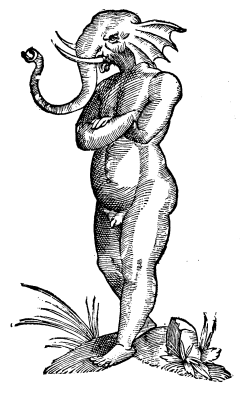
\includegraphics[scale=.5]{Goblin_3}
  \end{center}


\mybold{Goo}
	\mylist {
		\item 1st time:  You can turn yourself into a big pile of ... goo.  You are immune to physical (but not magical) damage, and you can't move or affect the environment in any way.
        \item 2nd time:  As above, but you can ooze around slowly (at about the pace of a slow walk)
        \item 3rd time:  Roll again
	}

\mybold{Harpy Claws}
	\mylist {
		\item 1st time:  You have sharp nails; you can climb dirt walls and can dig a small hole in soft soil
        \item 2nd time:  Your nails are distinct claws.  You can climb dirt and rough stone walls, and can dig a small hole in hard packed dirt. You can fight with your claws as Florentine weapons (Hard Brawl Stabbing weapon, d4)
        \item 3rd time:  Your claws are now talons.  You can make a small hole in stone, and can climb smooth ice or rock walls.  You can fight with your talons as Florentine weapons (Hard Brawl Stabbing weapon, d8)
        \item 4th time:  Roll again
	}
\mybold{Lie Can}
	\mylist {
		\item  1st time:  Once per Session, you can turn into a were-beast.  You tell the Arbiter what the beast is.  You can't use this Virtue while wearing armor.  Immediately drop anything you're holding, but gain the following additional abilities:  Berserk, +10 Flesh, Claws (Hard Brawl d8, Florentine), Regenerate 1 Flesh at the top of the Moment (unless you are struck with magic or silver).  
        \item  2nd time: Roll again
	}
\mybold{'nother Arm}
	\mylist {
		\item 1st time:  You get another arm.  It's pretty weak - you can't fight with it or anything, but it's useful for holding stuff
        \item 2nd time:  Your other arm is a lot stronger.  You can use it to hold a shield, or hang from something and keep your other arms free.
        \item 3rd time:  If your \DEX is d16 or greater, you can fight with a weapon in all 3 hands.  Treat as the same rules as Florentine, except the combined damage can't exceed d18.
        \item 4th time:  Roll again
	}
\mybold{Owl Eyes}
	\mylist {
		\item 1st time: You have giant owl eyes, granting you Dark Sight
        \item 2nd time: As above, plus you have Low Light Vision
        \item 3rd time: You can switch between Dark Sight, Low Light Vision, and Day Vision at will
        \item 4th time: Roll again
	}
\mybold{Pig Snout}
	\mylist {
		\item  1st time: You can smell any metal you choose (gold, silver, iron, etc) up to 1m away.
        \item  2nd time: As above, plus you can smell blood and flesh up to 50m away (100m if they are an Englishman)
        \item  3rd time: As above, plus you can smell magic on people, weapons, and objects
        \item  4th time: Roll again
	}
\mybold{Rat Tail}
	\mylist {
		\item 1st time: If a Monster's attack is about to cause you \mybold{physical} damage, you may immediately take a Combat Action and sacrifice your tail, taking no damage
        \item 2nd time: As above, plus the tail is strong enough for you to hang from
        \item 3rd time: As above, but you can use your tail as a whip.  The whips is a Fast Brawl weapon that deals d4 damage.  If you roll a 4, you can forgo damage and try to Disarm your opponent instead by \RB using your \DEX.
        \item 4th time: Roll again
	}


\mybold{Rooty}
	\mylist {
		\item  1st time: You can sprout roots from your hands and/or feet.  These roots can wrap around objects no wider than .5m, holding you in place
        \item  2nd time: As above, but the roots can wrap around things up to 2m wide
        \item  3rd time: As above, but the roots can dig into dirt or rock
        \item  4th time: Roll again
	}

\mybold{Shell}
	\mylist {
		\item 1st time:  A shell of hard chitin, granting you Soak: 1
        \item 2nd time:  The shell is now hard as quartz, granting you Soak: 2
        \item 3rd time:  The shell is as hard as diamond, granting you Soak: 3
        \item 4th time:  Roll again
	}


\mybold{Skin Bag}
	\mylist {
		\item 1st time:  You have a pouch ... somewhere ... on your body.  The pouch is about the size of a cigar box - common sense should prevail what can be stored in it.
        \item 2nd time:  As above, but the pouch has a \mylink{Hammerspace}{keyword-hammerspace} aspect to it.  You can carry 1 Significant Item
        \item 3rd time:  As above, but you can now carry 10 Significant Items.
        \item 4th time:  Roll again
	}
\mybold{Smoky}
	\mylist {
		\item 1st time: Once per Session, you can turn your body ghostly and insubstantial during Combat.  Monsters must make an immediate Morale roll; further, you're granted a +4 Guard roll, and you are only struck by magic.
        \item 2nd time: You may turn insubstantial during Combat as above; in addition, outside of Combat, you can turn into smoke for d6 minutes (the Arbiter will time you).  You move slowly, but you can seep beneath doors, through cracks, and into chimneys. You can't seep into anyone's lungs, they cough you out right away. Weapons can't harm you, but certain spells or effects that disperse smoke (Arbiter's judgment) will cause you to become substantial.
        \item 3rd time:  Roll again
	}

\mybold{Spider Eyes}
	\mylist {
		\item 1st time:  You can't be \mylink{Blinded}{effect-blinded}
        \item 2nd time:  As above, plus you can't be Surprised
        \item 3rd time:  As above, plus you can see Invisible creatures, and Mirror Image has no effect on you.
        \item 4th time:  Roll again
	}

  \begin{center}
  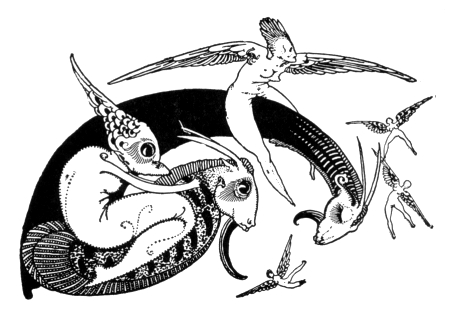
\includegraphics[scale=.5]{Goblin_4}
  \end{center}


\mybold{Sticky}
	\mylist {
		\item  1st time: You're generally ... sticky.  Like the adhesive on the back of a sticky note.  You could stick papers to yourself, and you won't lose your grip if you're climbing a rope or ladder
        \item  2nd time: You're now as sticky as tar.  You won't drop things that you're holding (you can't be disarmed).  You could stick a weapon to your body.  You can turn this stickiness "off" at will.
        \item  3rd time: You're now as sticky as sovereign glue.  You can't drop things you're holding unless you will it.  You can climb up a wall like a spider and hang from the ceiling like a fly (though you'd need to be naked).
        \item  4th time: Roll again
	}

\mybold{Tough'un}
	\mylist {
		\item 1st time: \myital{He was like a saddlebag with eyes!}  You look (and are) very tough.  You get a +2 to any rolls where you're trying to intimidate someone.  You don't take any damage from effects of mundane weather (snow, rain, sand, etc)
        \item 2nd time: As above, plus you add +4 to any \DEATH rolls
        \item 3rd time: As above, plus you gain +10 Flesh
        \item 4th time: Roll again
	}
\mybold{Tusky}
	\mylist {
		\item 1st time:  You grow a pair of small tusks.  The tusks act as if you're wearing a helmet.  If you should sunder them, they'll grow back after you take a Vacation.
        \item 2nd time:  As above, but your tusks are much bigger.  If you execute the \mylink{Bum Rush}{combat-deeds-bum-rush}, you can strike with your tusks as a Combat Action.  The tusks are Hard Brawl weapons that deal d6 damage.
        \item 3rd time:  As above, but your tusks are huge.  You like to decorate them with bands of iron and rings.  Your tusks are treated as Hard Brawl weapons that do d12 damage in a \mylink{Bum Rush}{combat-deeds-bum-rush}
        \item 4th time:  Roll again
	}


  \mysubsection{Gear}{night-children-virtues-gear}


\mybold{Bedlam Bag}
	\mylist {
		\item When you open the bag and turn it upside down, roll a d4 to see what falls out:  (1) a few thousand ball bearings; (2) a bomb with a countdown timer.  The bomb will explode at the bottom of the \mybold{next} Moment.  There's a 50/50 chance it's a dud (the Arbiter will roll in secret), but will deal 8d6 damage to everyone Close to it if it explodes (Save vs Doom for half damage).  The bomb can be thrown;  (3) a half dozen gremlins fall out and run in different directions, immediately causing as many problems as possible for Minutes; (d)  Bats. A lot.
	}




\mybold{Big Helm}
	\mylist {
		\item A giant helmet.  The helmet will protect you from being \mylink{Dazed}{gear-weapon-daze} and from certain Wounds and Beatings.  In addition, if a Monster's attack is about to cause you \mybold{physical} damage, you may immediately take a Combat Action to destroy the helmet, taking no damage.  The helmet is "fixed" at the start of next Session.
	}
\mybold{Big Pal}
	\mylist {
		\item Your big pal is .5m taller than you, looks extremely intimidating, and is very sensitive.  Big pal's feelings get hurt easily.  Big pal can carry you around and boost you up for hard to reach places.  In Combat, Big Pal likes to watch from the back and shout encouragement; however, if you are ever injured in Combat, your Big Pal will immediately join the fight.  Big Pal has 6 Flesh and gives you +4 to your Fight \RO.  You can put any damage you would normally take on Big Pal instead.  If Big Pal should die, another Big Pal shows up at the start of the next Session.
	}

  \begin{center}
  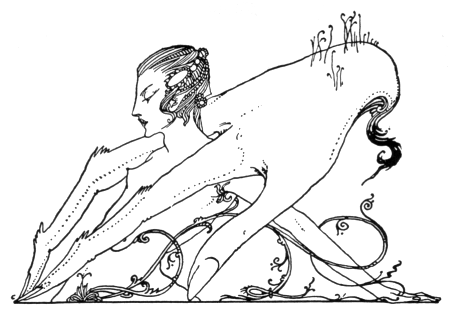
\includegraphics[scale=.5]{Goblin_5}
  \end{center}


\mybold{Big Shield}
	\mylist {
		\item A giant shield.  The shield should be treated as an additional suit of Light Armor (d4 \UD); however it takes 2 hands to use.  The shield is repaired the same way Armor is.
	}
\mybold{Bogeylatch}
	\mylist {
		\item  Once per Session, you can attach this doorknob to a hard surface and open a door 2m high, 1m wide, and .5m thick.  The door exists until someone closes it; the bogeylatch appears back in your pocket.
	}

\mybold{Bug Pal}
	\mylist {
		\item  You can ride it. If it dies, you find a new bug pal at the start of next Session.  Edible.
	}
\mybold{Devil Pen}
	\mylist {
		\item  Contracts signed with this pen (in blood) between two willing parties are magically enforced. Breaking the contract means the responsible party suffers a permanent Greater Curse which can only be removed by the other party in the contract.
	}
\mybold{Fly Rug}
	\mylist {
		\item  You and up to 4 allies can "ride" this flying carpet.  The rug can levitate up and down and can move forwards and backwards at a slow pace (about walking speed).  The Fly Rug has no handles, so be careful you don't get knocked off.
	}


\mybold{Gobbomb}
	\mylist {
		\item \myital{Anytime I had a problem and I threw a Molotov cocktail, boom! Right away, I had a different problem}  At the start of the Session, you create 3 explosive grenades.  These are Fast Throw weapons that deal 3d6 damage to everything Close to their point of explosion (Save vs Doom for half damage).  Throwing a grenade is a Combat Action.  The grenades will also set flammable things on fire.  Every grenade has a 1-in-4 chance of being a dud (rolled in secret by the Arbiter).  If you don't use the grenades by the end of the Session, they're all duds.
	}
\mybold{Gobsword}
	\mylist {
		\item You gain a weapon appropriate for your species: a pair of Norn scissors, a giant tooth through a club, the mandible of a predatory insect - tell the Arbiter what it is.  The weapon is a Fast Brawl weapon that does d8 damage and is magic.
	}
\mybold{Gremlin Tools}
	\mylist {
		\item  Once per Session, you can use the Gremlin tools to do one of the following:  (a) remove a Trivial or Minor Sigil; (b) "repair" 4 points of Flesh damage (not pretty); (c) repair a suit of Armor to its \MAX \UD; (d) "fix" something that's broken (Arbiter's discretion)
	}
\mybold{Hole}
	\mylist {
		\item  It's a hole you can fold up like a handkerchief.  The hole can be laid flat on any surface, but it has to stick there (so you'll have to get creative if you want to hang it from the wall or ceiling).  The hole is 500 cm wide but 3m deep.  Anything you put in here is considered to be in \mylink{Hammerspace}{keyword-hammerspace}  
	}
\mybold{Kazoo}
	\mylist {
		\item  Once per Session, you can put on a little kazoo concert.  Pick 1:  (a) purge a Mental or Spiritual Wound from someone; (b) during a Breather, bring everyone to full Grit; (c) end all Markovian effects Close to you; (d) restore 1 point of Flesh to everyone Close to you (friend or foe).  If you actually play the kazoo, pick 2.
	}



\mybold{Kissy Lips}
	\mylist {
		\item  A tube of very bright coral lipstick.  Once per Session, you can apply this lipstick and do one of the following:  (a) tell everyone about the interesting things in a room you're in, even if hidden from view ("there's a secret door in the north wall, a magic dagger hidden in the chimney, and a spider waiting to ambush us in the corner."); (b) tell effortless and undetectable lies for d6 Minutes;  (c) Charm everyone Close to you with a risqué performance (Save vs Doom or Charmed for as long as you perform); (d) whistle a tune that removes all Markovian effects on Allies Close or Nearby.
	}


\mybold{Little Buddy}
	\mylist {
		\item  A little kobold buddy. He can't do much except hold a light source.  Unquestionably loyal and extraordinarily stupid.  If he dies, you find a new friend the next day.  Edible.
	}
\mybold{Magic Beans}
	\mylist {
		\item At any time, you can water your Magic Beans and grow them.  Roll a d24 on this table; that piece of Gear grows from the Magic Beans.  If you roll a piece of Gear you already have - too bad, nothing happens.
	}
\mybold{Mirror Mirror}
	\mylist {
		\item Once per Session, you can reach into the Mirror Mirror and pull out a copy of an object reflected in the mirror.  The object that you pull out must be within reach of the mirror (as if it were a window), small enough to fit through the mirror (as if it were a window) and can’t weigh
more than 10kg. The mirror object looks and feels exactly like the object it copied, though it is a mirror image (so if you were to copy a book, the text would be backwards). You can’t copy any magical properties of the object, and you can only duplicate objects, not living things. The object exists for Minutes. If the object suffers a solid blow, it pops like a bubble.
	}

\mybold{Packpack}
	\mylist {
		\item  Giant, colossal backpack that only you can wear.  You can reach into this backpack and produce any mundane item (at the Arbiter's final discretion).  The object can't be valuable in and of itself (no pulling out gems or jewels) and has to be smaller than a human arm (daggers and short swords OK, polearms not so much).  Additionally, you can store 25 Significant Items in the backpack as if they were in \mylink{Hammerspace}{keyword-hammerspace}.  The backpack doesn't affect your \MD in any way. 
	}

\mybold{Red Shoes}
	\mylist {
		\item  Once per Session, you can click the heels of your Red Shoes together to undo \mybold{any} die roll that hits the table.  The person who rolled immediately re-rolls.  You have to have feet to use the Red Shoes.
	}
\mybold{Skelly Key}
	\mylist {
		\item Once per Session, you can open any mundane locked thing.  
	}

  \begin{center}
  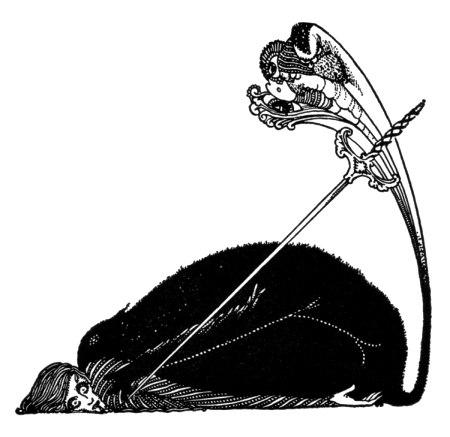
\includegraphics[scale=.5]{Goblin_6}
  \end{center}


\cbreak

\mybold{Spinny Wheel}
	\mylist {
		\item  Once per Session, you can use the Spinny Wheel when taking a \mylink{Bivouac}{combat-resting-bivouac} to produce one of the following: (a) 10 gold coins (doesn't count for XP).  Requires straw; (b) a single dose of any Iron or Silver Toxin or Sera.  The dose is delivered through the spindle; (c) an unraveling spool of thread that shows you the most direct way out of where you are; (d) a story that enchants all of your Allies, granting +6 Grit (even above their \MAX)
	}
\mybold{The Crew}
	\mylist {
		\item  A crew of goblins, kobolds, orcs, and other unsavories follows you around (d4+2 to start).  Every 2 members of the Crew (rounded down) grant you +1 to all \RO and \RS attempts.  Each Crew member requires a Provision roll when taking a \mylink{Bivouac}{combat-resting-bivouac} (though they are cannibalistic so there's some cost cutting opportunities).  They are loyal, loud, and extraordinarily stupid.  Sneaking up on people is out.  Your crew is always between 2 and 10 members.  If you ever get to 0 crew members, 2 crew members show up next Session - otherwise, you gain 1 crew member each Session, up to 10 crew.
	}



\mybold{Trunk Pal}
	\mylist {
		\item A small bureau that follows you around on hundreds of tiny feet.  Surprisingly fast.  Can store up to 25 Significant Items for you and obey simple commands.  Will "give" you an item stored in it at your immediate request. If it gets destroyed, you find it leaning over you when you wake up next Session - but there's a 50/50 chance each Significant Item in it doesn't make it back (roll for each)
	}
\mybold{Vorpal Sword}
	\mylist {
		\item  A beautiful jewel encrusted sword of extraordinary sharpness.  The Vorpal Sword is a Hard Brawl weapon that deals d8 damage and is magic.  The damage die explodes.  If you ever do 20+ points of damage with the sword, the victim is decapitated unless they make a Save vs Doom.
	}

\newpage

\mysubsection{Snags}{night-children-complications}

\mybold{Backwards}
	\mylist {
		\item  You're put together backwards, meaning your feet or arms go the other way.  You get easily confused with directions - if you're by yourself, you automatically get lost
	}
\mybold{Bad Mouth}
	\mylist {
		\item   No one can understand your accent until they've deal with you for awhile.  You're Allies understand you, but no one else does.
	}
\mybold{Bumpback}
	\mylist {
		\item   Doesn't affect your movement or anything, but everyone always assumes you're the party's assistant / torch-bearer / etc.  You don't get much respect.
	}
\mybold{Dirty}
	\mylist {
		\item  You can't own nice things.  Clothing you wear becomes almost instantly soiled, weapons rusty, armor squeaky.  It doesn't have any mechanical effect, but you're not permitted in polite society
	}
\mybold{Fat}
	\mylist {
		\item  You're a little round around the edges.  Your extra weight takes up 1 Significant Item slot.
	}


\mybold{Glowy}
	\mylist {
		\item  You have a slight ... glow about you. Makes it almost impossible to hide unless you're completely covered by thick cloth. 
	}
\mybold{Me Cold!}
	\mylist {
		\item  You get cold very easily.  You'll refuse to go somewhere if it's too cold.
	}
\mybold{Me Hot!}
	\mylist {
		\item You get hot very easily.  You'll refuse to go somewhere if it's too hot.
	}
\mybold{Me Hungry!}
	\mylist {
		\item You're always starving; you need to roll your Provisions twice when you Bivouac
	}

\mybold{Me Tired...}
	\mylist {
		\item You sleep very deeply.  It takes an extra Action to wake you up.
	}
\mybold{Pinhead}
	\mylist {
		\item You have a really, reaalllly tiny head.  People laugh awkwardly.  You can't wear a Helmet (except for a Big Helm).
	}
\mybold{Smell Yummy}
	\mylist {
		\item You smell delicious to Monsters.  They'll go for you first in a fight.
	}

\mybold{Stealy}
	\mylist {
		\item You like to steal stuff.  You're compelled to try to steal something once a Session.
	}
\mybold{Weird Voice}
	\mylist {
		\item You have a weird voice (roll again if you're not comfortable role-playing this)
	}
\mybold{Who That?}
	\mylist {
		\item You have absolutely no memory of faces, except for your Allies.
	}


